
% \chapter{Introduction}
\chapter{Introducere}
\label{cap:Introducere}
 \section{Contextul lucrării}
Conform statisticilor Poliției Române \cite{politia_romana}  în anul 2017 în România au fost 8624 de accidente rutiere în care 1951 oameni și-au pierdut viața iar 8172 oameni au fost răniți grav. Dacă ne uităm pe statiscticile întregii lumi \cite{WHO}  vedem că cca. 1,3 milioane de oameni mor anual în accidente rutiere.\newline
Statisticile de accidente ne arată că  în 94\% dintre toate accidentele are rol și eroarea umană, iar 76\% sunt cauzate numai de eroarea umană.
 Fred Wegman și Letty Aarts  în \cite{SWOV} prezintă că în accidentele rutiere cei mai vulnerabili sunt pietonii (în special copiii) și bicicliștii aceștia fiind neprotejați. Locul doi pe lista de top a vulnerabilității o țin conducătorii de motociclete, mopeduri, etc. pentru că ei sunt numai parțial protejați (\ref{fig:lethalities}).\newline

%image of table with vulnerabilities in age and transport modes categories
\begin{figure}[h!]
    	\centering
	\captionsetup{justification=centering, margin=2cm}
	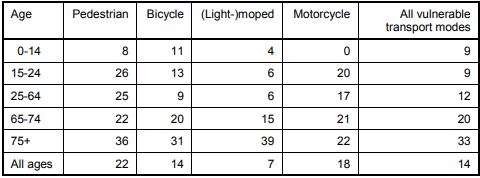
\includegraphics[width=0.8\textwidth]{figures/lethality_rates.png}
	\caption{Numărul de persoane implicate separate după vârstă și modul de transport pe 100 accidente serioase \cite{SWOV}}
	\label{fig:lethalities}
\end{figure}

Numerele acestea ridicate motivează aspirația noastră spre a construi sisteme inteligente care pot ne să ajute la evitarea dramelor rutiere. Avem două așteptări cruciale față de un asemenea sistem inteligent: să funcționeze în timp real și să aibă o rată foarte ridicată de detecție corectă. Alarmele false sunt costisitoare și iritante pentru persoanele aflate în vehicul, iar greșelile în care sistemul nu recunoaște pericolul pot avea consecințe fatale.\newline
Pentru luarea deciziilor, sistemul trebuie să obțină informațiile necesare din scenele de trafic, iar acest lucru se poate face prin mai multe modalități; în \cite{car_sensors}  Gert Rudolph și Uwe Voelzke prezintă cele mai folosite metode de colectarea informațiilor pentru mașini autonome:
\begin{itemize}
	\item Camere video 360$^\circ$: fără îndoială imaginile video conțin peste 90\% din informația de care are nevoie un conducător uman dar sunt potrivite și pentru conducerea vehiculelor autonome. Este critic ca camerele folosite să se descurce în toate condițiile de luminare și stare atmosferică.
	\item Radio Detection And Ranging (RADAR): sistemele ADAS (Advanced Driver Assistance Systems) necesită un număr mare de senzori, aceștia facând o contribuție la conducerea autonomă. RADARele se folosesc în asistarea parcării, în recunoașterea situațiilor în care este nevoie de frânare imediată, măsurarea distanțelor, etc.
	\item Light Detection And Ranging (LiDAR): LiDAR este un sistem bazat pe laser, relativ nou în contextul vehiculelor autonome. Pe lângă \textit{transmitter} (laser) este nevoie și de un \textit{receiver} foarte sensibil. Folosit în primul rând pentru măsurarea distanțelor obiectelor staționare și a celor în mișcare, sistemul folosește proceduri speciale pentru construirea unei imagini 3D a obiectelor detectate.
	\item Sonare ultrasonice, GPS, senzori termale, etc.
\end{itemize}
Deși pentru oameni recunoașterea actorilor dintr-o scenă de trafic este o problemă trivială, pentru sistemele informatice este una dificilă, aceștia având nevoie de algoritmi isteți. Condițiile de luminare, vizibilitate precum și trăsăturile obiectelor (rotație, mărime, mișcare, culorile, etc.) sunt factori care îngreunează recunoașterea actorilor dintr-o scenă.

\section {Tema Lucrării}
Tema lucrării de față este recunoașterea actorilor în imaginile captate din scene de trafic urban folosind inteligență artificială. Astfel se află la intersecția a două domenii care au primit foarte multă atenție recent: viziune artificială și inteligență artificială; cu algoritmi de procesare de imagini se vor extrage informații din imagini, iar cu ajutorul unei rețele neuronale se va face detectarea obiectelor în imaginile prelucrate precum și segmentarea semantică a imaginilor.\newline
De ce rețelele neuronale (convoluționale)? Putem să motivăm această decizie cu un mic exemplu luat din cadrul recunoașterii obiectelor dintr-o imagine: să propunem că problema noastră este de a face un program care poate recuoască un cub simplu, fără nicio textură specială pe o imagine. Chiar și acest obiect simplu introduce mii de probleme dacă folosim metode tradiționale: obiectul poate fi mai mic sau mai mare, se poate roti; și diferitele condiții de luminare pot să încurce programul nostru, precum și zgomotul din imagine. Și ce se întâmplă dacă vrem să recunoaștem un cub care poate să aibă și textură? Durere de cap! Am avea nevoie de o cantitate imensă de pre-procesări ca să putem să tragem concluzii uniforme.\newline
Aici intră în "imagine" puterea rețelelor neuronale. Acestea nu au nevoie de nicio trăsătură unică și specială care diferențiază o categorie de obiecte de o altă categorie. Dacă rețeaua neuronală are un set de antrenare variat și destul de mare, poate să tragă concluzii și să facă generalizări despre obiecte acestea fiind imune la zgomote; funcționând asemănător cu cortexul vizual animalelor, o rețea neuronală antrenată este greu de înșelat.\newline
Domeniul exact al temei este clasificarea imaginilor, detecția obiectelor și segmentarea semantică a imaginilor folosind rețele neuronale \textit{convoluționale}(CNN).
%image presenting image classification, detection and segmentation
\begin{figure}[h!]
    	\centering
	\captionsetup{justification=centering, margin=2cm}
	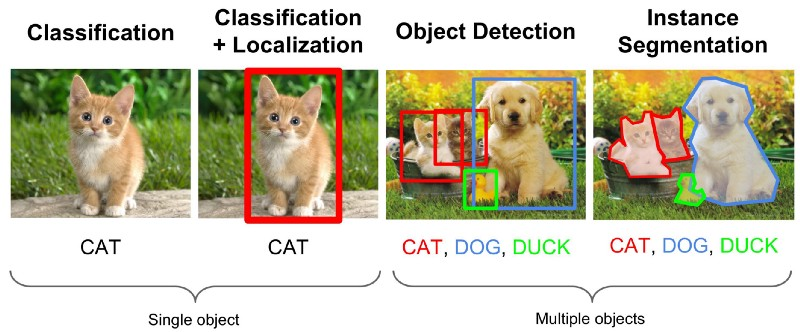
\includegraphics[width=0.9\textwidth]{figures/class_detect_segment.jpeg}
	\caption{Clasificare de imagine, localizare, detecție de obiecte, segmentare semantică \cite{class_detect_segment}}
	\label{fig:class_detect_semgent}
\end{figure}
Dacă ne uităm pe figura - putem să înțelegem ce înseamnă aceste concepte și că vorbim de trei procese diferite:
\begin{itemize}
	\item \textbf{Clasificarea} unei imagini constă în atribuirea unei etichete (label), specificarea categoriei de obiecte în care se încadrează obiectul reprezentat în imaginea respectivă,
	\item Când găsim dreptunghiul înăuntrul căreia se afla obiectul respectiv, vorbim despre \textbf{detecție de obiect},
	\item \textbf{Segmentarea semantică} este procesul prin care pentru fiecare pixel îi atribuim un obiect.
\end{itemize}
